\documentclass[a4paper,10pt,twoside]{book}
\usepackage[italian]{babel}
% \usepackage{lmodern}
\usepackage[T1]{fontenc}
\usepackage[utf8]{inputenc}
%  \usepackage[sc]{mathpazo}
 \usepackage{mathpazo} % Supporto matematico al font Palatino. Imposta automaticamente il font?
 \linespread{1.05} % palatino needs more space between lines

% FANCY THINGS
\usepackage[Lenny]{fncychap} %Titolo dei capitoli figo
  \ChRuleWidth{2pt} %Spessore delle linee di fncychap
  \ChNameVar{\fontsize{14}{16}\usefont{T1}{ppl}{m}{n}\selectfont} %Nome ``capitolo'' viene in Palatino, medium, normale. Valuta anche il bold normale.
%   \ChNameVar{\fontsize{14}{16}\selectfont} %Nome ``capitolo'' viene in Palatino, medium, normale. Valuta anche il bold normale.

\usepackage[babel]{csquotes}
\usepackage[hyperref,style=alphabetic]{biblatex}
\bibliography{references}

\usepackage{graphicx} % Allows for eps images
\usepackage[colorlinks=true, linkcolor=blue,citecolor=magenta,filecolor=green,urlcolor=cyan]{hyperref}	% links to references
\usepackage{color}	% colors
\usepackage{booktabs}	% good tables
\usepackage[strict]{chngpage}
\usepackage{enumerate}
\usepackage{enumitem}
\usepackage{algorithmic}
\usepackage{microtype} %% VERY VERY USEFUL FOR CORRECT HYPHENATION
\usepackage{setspace}
% \singlespacing


% MATH STUFF
\usepackage{amsfonts}
\usepackage{amsmath} % AMS Math Package
\usepackage{amsthm} % Theorem Formatting
\usepackage{amssymb}	% Math symbols such as \mathbb
% \numberwithin{equation}{chapter}

\theoremstyle{definition}
\newtheorem{definition}{Definizione}[chapter]

\theoremstyle{plain}
\newtheorem{theorem}{Teorema}[chapter]
\newtheorem{lemma}[theorem]{Lemma}
\newtheorem{proposition}[theorem]{Proposizione}
\newtheorem{corollary}[theorem]{Corollario}

\theoremstyle{definition}
\newtheorem{remark}{Osservazione}[chapter]
\newtheorem{note}[remark]{Nota}
\newtheorem{case}[remark]{Caso}

% \newenvironment{proof}[1][Dimostrazione]{\begin{trivlist}
% \item[\hskip \labelsep {\bfseries #1}]}{\end{trivlist}}

% \newenvironment{teorema}[1][Teorema]{\begin{trivlist}
% \item[\hskip \labelsep {\bfseries #1}]}{\end{trivlist}}

% \newenvironment{definition}[1][Definizione]{\begin{trivlist}
% \item[\hskip \labelsep {\bfseries #1}]}{\end{trivlist}}

% \newenvironment{example}[1][Esempio]{\begin{trivlist}
% \item[\hskip \labelsep {\bfseries #1}]}{\end{trivlist}}

% \newenvironment{remark}[1][Osservazione]{\begin{trivlist}
% \item[\hskip \labelsep {\bfseries #1}]}{\end{trivlist}}

% \newcommand{\qed}{\nobreak \ifvmode \relax \else
%       \ifdim\lastskip<1.5em \hskip-\lastskip
%       \hskip1.5em plus0em minus0.5em \fi \nobreak
%       \vrule height0.75em width0.75em depth0.25em\fi}


% Immagine di background nel frontespizio
\usepackage{eso-pic}
\newcommand\BackgroundPic{%
\put(0.,110){%
\parbox[b][1.2\paperheight]{0.5\paperwidth}{%
\vfill
\centering
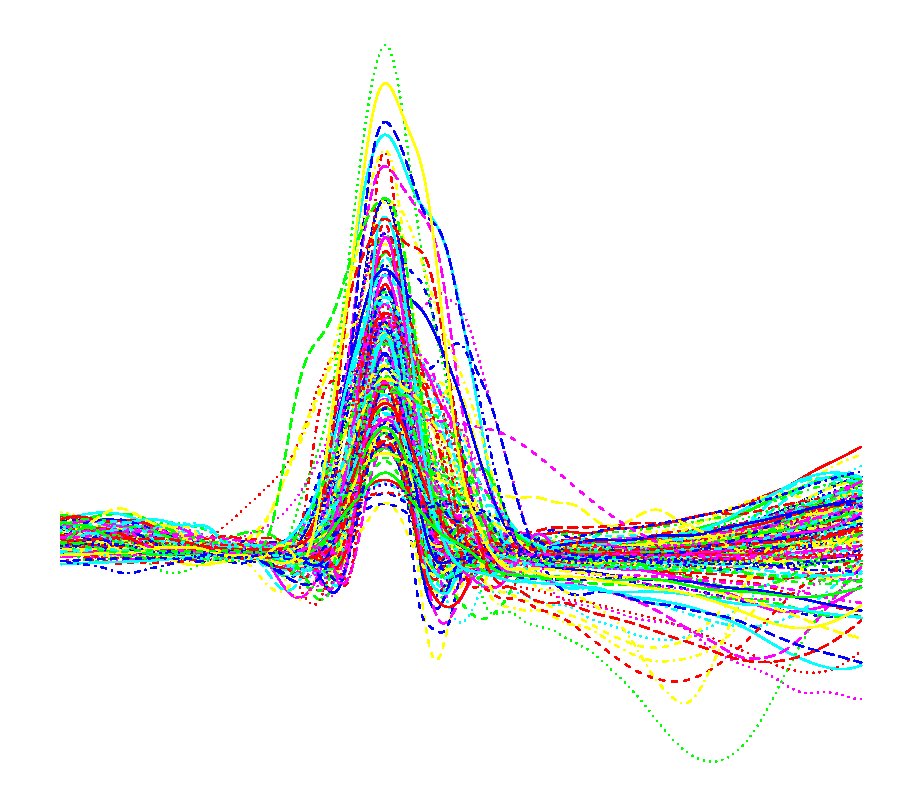
\includegraphics[width=\paperwidth,height=\paperheight,%
keepaspectratio]{img/matplot_trimmed}%
\vfill
}}}